  % Background: Syntax, type systems, and operational semantics
\newcommand{\param}[1]{\langle #1 \rangle}
\newcommand{\syn}[1]{\mathsf{#1}}


  In the formal study of a programming langugage, one may define a language
  in three parts: syntax, type system, and operational semantics.
  \begin{itemize}
    \item The {\em syntax} is written in the form of a (usually)
      context-free grammar describing the allowable expressions. One
      sometimes distinguishes between {\em concrete syntax}, the literal
      program tokens that the programmer strings together in the act of
      programming, and {\em abstract syntax}, the normalized ``syntax
      tree'' structures that ultimately get interpreted. 
    \item An {\em operational semantics} defines how runnable programs
      (e.g. a function applied to an argument) {\em reduce} to values. This
      part of the definition describes how actual computation takes place
      when programs in the language are run. It is important to note that
      the operational semantics need not reflect the actual {\em
      implementation} of the language, nor is it specific to a ``compiled''
      versus ``interpreted'' understanding of the language: it is simply a
      mathematical specification for how any compiler or interpreter for
      the language should behave.
    \item A {\em type system} further refines the set of syntactically
      valid expressions into a set of {\em meaningful} expressions, and provides
      a mapping between an expression and an approximation of its meaning.
      Type systems are usually designed in conjunction with the operational
      semantics to have the property that every expression assigned a
      meaning by the type system should have a well-defined runtime
      behavior. In practice, however, type systems can only approximate
      this correspondence. Some err on the more permissive side--e.g.
      C's type system will permit invalid memory accesses with no
      language-defined behavior--and some err on the more restrictive side,
      e.g. Haskell's type system does not permit any untracked
      side-effects, at the expense of easily authoring e.g. file input/output
      (without first learning the details of the type system).
  \end{itemize}
  
  Providing a formal language definition in programming languages research
  has several purposes. One is that it enables researchers to explore
  and prove formal properties of their language, such as {\em well-typed
  programs don't go wrong}, or in a language for concurrency, a property
  like deadlock freedom. However, an even more crucial advantage of a
  language specification is not mathematical rigor but human capacity to do
  science. A language definition is a {\em specification}, similar to an
  application programmer interface (API) or an IEEE standard: it describes
  an unambiguous interface to the language along an {\em abstraction
  boundary} that other human beings may access, understand, and implement,
  without knowing the internals of a language implementation.  It is a
  necessary component of reproducibility of research, and it allows
  researchers to build on each other's work. We believe that an embrace of
  the formal specification in games research can play a similarly important
  function.

  \begin{table}
  \begin{tabular}{l|ll}
    PL concept & Game concept\\
    \hline
    Syntax & Recognized player intents & (Section \ref{sec:syntax})\\
    Operational semantics & Game mechanics & (Section \ref{sec:opsem})\\
    Type system & Contextual interface & (Section \ref{sec:typesys})\\
    Straight-line programs & Play traces & (Section \ref{sec:traces})\\ 
    General programs & Player skills & (Section \ref{sec:skills})
    \\
    \hline
  \end{tabular}
%  \caption{Languages for player-game interfaces: Formal decomposition
 %   (left) and informal correspondances (right).}
  \caption{Player intent languages: 
    \\
    Formal decomposition (left) and correspondances (right).}
  \label{tab:correspondence}
  \end{table}

  Having provided loose definitions of these terms, we now wish to draw out
  the analogy between a {\em language} specification and a {\em game}
  specification. To treat a game in this manner, we wish to consider player
  affordances and actions, as well as their behavior (mechanics) in the
  context of the game's running environment. We summarize the components of
  this correspondence in Table~\ref{tab:correspondence}.

  \newcommand{\cmove}{\mathsf{move}}
  \newcommand{\ctake}{\mathsf{take}}
  \newcommand{\ccollect}{\mathsf{collect}}

  We will use as a running example a minimal virtual environment with two
  player actions: (1) movement through a discrete set of rooms in a
  pre-defined map ($\cmove$); (2) acquiring objects placed in those rooms to store in
  a player inventory ($\ctake$).  We consider five (somewhat aribitrary)
  possibilities in the design space of interfaces for such a game,
  summarized visually in Figure~\ref{fig:uis}:

  \begin{itemize}
   \item {\bf Point-and-Click:} A first-person viewpoint interface where the
     meaning of each click is defined based on the region the cursor falls
     in. Clicking near any of the four screen edges moves in that
     direction; clicking on a sprite representing an item takes it.
  \item {\bf Bird's-Eye:} A top-down viewpoint interface where the player can see multiple
    rooms at once, and can click on rooms and objects that are far away,
    but those clicks only do something to objects in the same room or
    adjacent rooms.
  \item {\bf WASD+:} A keyboard or controller-based interface with
    directional buttons (e.g. arrow keys or WASD) move an avatar in the
    correspondingi direction, and a separate key or button expresses
    the $\ctake$ action, which takes any object in the same room. (This
    interface may be used for either of the two views described above.)
  \item{\bf Command-Line:} The player interacts by typing free-form text, 
    which is then parsed into commands, such as \verb|take lamp| and \verb|move north|.
  \item{\bf Hypertext}: A choice-based interface where all available options are
    enumerated as textual links from which the player chooses.
  \end{itemize}

  \begin{figure*}
    \begin{tabular}{cc}
      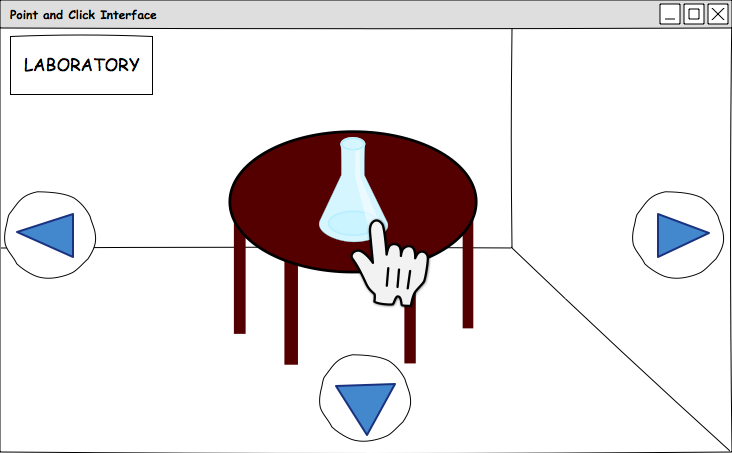
\includegraphics[height=0.2\textheight]{../uis/point-and-click.png} &
    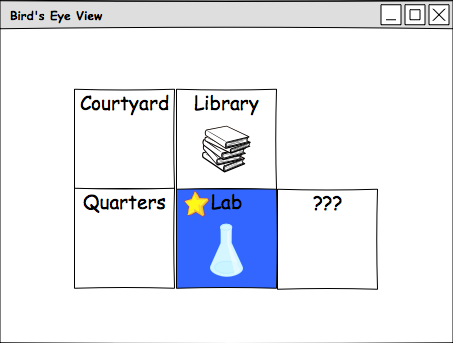
\includegraphics[height=0.2\textheight]{../uis/bev-color.png}
    \\
    Point-and-click & Bird's eye view/WASD+\\
    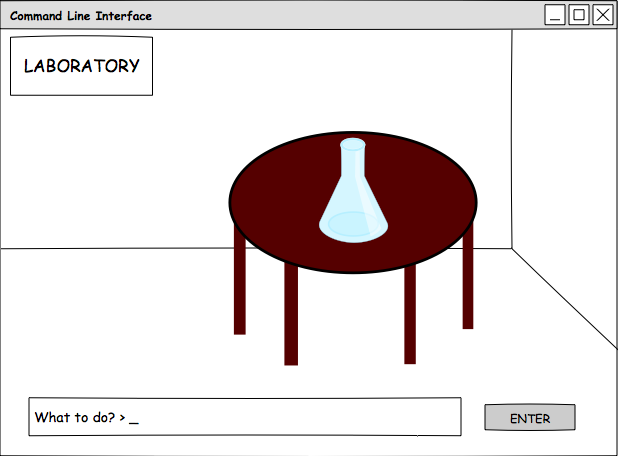
\includegraphics[height=0.2\textheight]{../uis/parser.png} &
    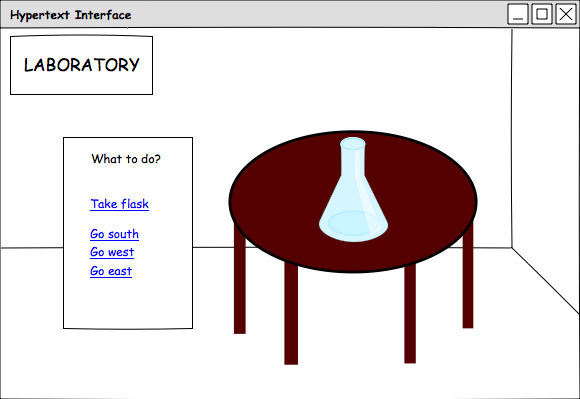
\includegraphics[height=0.2\textheight]{../uis/hypertext.png}\\
    Command-line & Hypertext
  \end{tabular}
  \caption{Four different user interfaces for the move/take game.}
  \label{fig:uis}
  \end{figure*}

  In the following sections, we will consider these possibilities in light
  of design choices relevant to the specified aspect of PL design.

  \section{Player intent as syntax}
  \label{sec:syntax}


%   \begin{figure*}
%     \begin{tabular}{|l|c|}
%       \hline
%       Language layer   & $\syn{move}(dir)$, etc. (XXX) \\
%       \hline
%       Affordance layer &
%         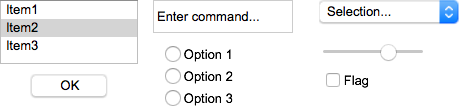
\includegraphics[width=0.5\textwidth]{ui-elements.png}\\
%       \hline
%       Device layer & 
%         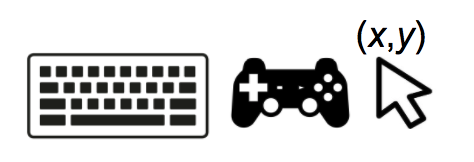
\includegraphics[width=0.4\textwidth]{control-devices.png}\\
%       \hline
%     \end{tabular}
%     \caption{XXX caption}
%     \label{fig:layers}
%   \end{figure*}
% 
% 
%   The {\em syntax} of a game is its space of recognized player commands.
%   However, this statement alone is imprecise: what counts as a {\em
%   command}, and what counts as {\em recognition}? Consider the
%   stratification of abstraction layers in Figure~\ref{fig:layers}: on the
%   hardware device level (which we consider out of scope for this paper),
%   the player issues a command by pressing, tapping, twisting, etc. 
%   physical buttons, keys, screens, and other tactile or embodied
%   affordances. This layer contends with the interactions between the
%   player's physical body and the game system. At the next layer up are
%   software affordances, or ``UI (user interface) elements:'' buttons,
%   sliders, menus, and other on-screen widgets that serve both to cue the
%   player ``interact with this'' and to {\em limit} the space of possible
%   hardware interactions (e.g. mouse clicks) to those that are relevant to
%   the particular software (e.g. buttons, check-boxes). Finally, the {\em
%   language} layer is closest to the game's mechanics themselves: the
%   recognized verbs, nouns, and other data relevant to a diagetic {\em
%   intent} that the player wishes to carry out.
% 
%   The two processing steps in this pipeline---device to affordance, and
%   affordance to language---resemble the distinction between concrete and
%   abstract syntax. An important difference between the two levels is
%   whether {\em context matters}: the keys on a keyboard may be pressed at
%   any time during a player's interaction with a computer; context within
%   the game world does not restrict their use. On the other hand, which menu
%   options are available may depend a great deal on context: if a player has
%   opened their inventory, different options may be available from those
%   available when looking at, say, an overworld map. Correspondingly,
%   context-independent actions are probably carried out
%   repeatedly---pressing arrow keys and space in a PC platformer using those
%   keys as controls, for example. On the other hand, their interpretation
%   one layer up---``jump onto the transport platform'' or ''fall down onto
%   (a specific) enemy NPC''---only make sense in very specific game world
%   contexts and are infrequently (or perhaps never) repeated.
% 
%   Where to draw the line between concrete and abstract is largely a matter
%   of choice that will determine how we can view and analyze a game.
%   In the following examples, we describe concrete syntax in terms of
%   anything a player can do that the game's audiovisual interface suggests
%   might be possible: e.g. if a mouse cursor is displayed whenever the
%   player moves the mouse, then we consider a mouse click anywhere on the
%   screen to be part of the concrete syntax. If a player is allowed to type
%   arbitrary text (or speak aloud arbitrary phonemes), and the game
%   interface displays or repeats back what the player said, then we consider
%   the concrete syntax to be those arbitrary sequences of characters or
%   phonemes.
% 
%   At the abstract layer, we 
%   

  The {\em syntax} of a game is its space of recognized player intentions.
  Note that {\em intention} is different from {\em action} in the sense
  that we don't necessarily expect each well-formed intention to change
  anything about the game state: a player can intend to move north, but if
  there is no room to the north of the player when she expresses this
  intent, no change to the game's internal state will occur. Nonetheless,
  depending on the design goals of the game, we may wish to recognize this
  as a valid intent so that the game may respond in some useful way (e.g.
  with feedback that the player cannot move in that direction).
  
  In our example game, the choice of syntax answers questions such as: can
  the player click anywhere, or only in regions that have meaning? Can the
  player type arbitrary commands, or should we provide a menu or
  auto-complete text so as to prevent the player from entering meaningless
  commands?  In PL, we can formalize these decisions by describing an {\em
  abstract syntax} for our language, which is typically assumed to be
  context-free and thus specified as a Bachus-Naur Form (BNF) grammar. Our
  examples below follow the interfaces shown visually in
  Figure~\ref{fig:uis}.
  
  \textbf{WASD+ Interface}:
  One way of writing the BNF for the WASD+ interface is:
  %
  \begin{eqnarray*}
  direction &::=& \mathsf{north} \mid \mathsf{south} \mid \mathsf{east}
    \mid \mathsf{west} \\
  intent &::=& \cmove \langle direction \rangle \mid \ccollect
  \end{eqnarray*}
  %
  The hardware interface maps onto this syntax quite directly:
  each arrow key maps onto a $\cmove$ action in the corresponding
  direction, and the specified other key maps onto $\ccollect$.

  \textbf{Bird's Eye View Mouse Interface}:
  On the other hand, a clicking-based interface to a top-down map could
  enable the player to click on any room on the map and any item within a
  room. This syntax would look like:
  %
  \begin{eqnarray*}
    room   &::=& \syn{courtyard} \mid \syn{library} \mid \syn{quarters}
              \mid \syn{lab}\\
    item   &::=& \syn{flask} \mid \syn{book}\\
    entity &::=& room \mid item\\
    intent &::=& \syn{click}\param{entity}
  \end{eqnarray*}
  %
  Note that this syntax, compared to that for WASD+, describes a larger set
  of possible utterances, even though it has the exact same set of
  permitted game behaviors (a player may only move into adjacent rooms and
  take items that share a room with them). 

% XXX make this point at the end of the section
%   The {\em size} of the player
%   intent language, i.e. the number of distinct intents it is possible to
%   form and express through the game language, constitutes a significant
%   aspect of the game design. A game with fewer expressible intents might
%   feel easier, and conversely less exploratory: the player is only allowed
%   to speak utterances that the game is guaranteed to validate. 

  \textbf{Command Line Interface}:
  The command-line interface would have an even larger space of expressible
  utterances if we consider all typed strings of characters to be valid
  expressions, but that syntax is too low-level for linguistic
  considerations. Supposing we interpose a parsing layer between arbitrary
  typed strings and syntactically-well-formed commands, we can define the
  abstract syntax as follows (where $direction$ and $item$ are assumed to
  be defined as they were in the previous examples):
%
  \begin{eqnarray*}
    intent &::=& \cmove\param{direction} \mid \ctake\param{item}
  \end{eqnarray*}
%
  Assuming the player ``knows the language,'' i.e. knows that $\cmove$
  and $\ctake$ are valid commands, and in fact the {\em only} valid
  commands, and assuming that she knows how to map the visual affordances
  (e.g. image of the flask) to the typed noun (e.g. \verb|flask|), the
  experience afforded by this interface is quite similar to the WASD+
  interface. The main difference is that the player must specify an {\em
  argument} to the $\syn{take}$ command, asking the player to formulate a
  more complete (and unambiguous) intent by actually naming the object she
  wishes to take.

%   When a player sees an empty command prompt as an interface to a game, she
%   may try using another language she knows, such as one used in classic
%   interactive fiction that recognizes a wide space of valid imperative
%   sentences:
%   \begin{eqnarray*}
%     intent &::=& iverb \mid
%                  tverb\param{noun} \mid
%                  \syn{go}\param{direction} \\
%              &\mid& \syn{put}\param{noun}\syn{\ on}\param{noun} \\
%              &\mid& \syn{strike}\param{noun}\syn{\ with}\param{noun}\\
%              &\mid& \hdots\\
%     iverb &::=& \syn{look} \mid \syn{listen} \mid \syn{wait} \mid \hdots\\
%     tverb &::=& \syn{take} \mid \syn{examine} \mid \syn{drop}\mid \hdots
%   \end{eqnarray*}



  \textbf{Hypertext interface}:
  Finally, we consider the intent language for the hypertext interface.
  This is one of the most difficult interfaces to formulate in linguistic
  terms, because it either requires that we formalize link selection in an
  acontextual way (e.g. as a numeric index into a list of options of
  unknown size) or that we formulate each link {\em from each page} as its
  own separate command, each of which has meaning in only one specific game
  context (namely, when the player is on the page containing that link).
  The former feels like a more general formulation of hypertext that is not
  relevant to any particular game, and since we are aiming to provide a
  correspondence between specific games and languages, we opt for the
  latter:
  %
  \begin{eqnarray*}
    intent &::=& \syn{select}\param{choice}\\
    choice &::=& \syn{take\_flask\_from\_lab}\\
           &\mid& \syn{take\_book\_from\_library}\\
           &\mid& \syn{go\_south\_from\_lab} \\
           &\mid& \syn{go\_east\_from\_lab} \\
           &\mid& \syn{go\_west\_from\_lab} \\
           &\mid& \syn{go\_north\_from\_library} \\
           &\mid& \hdots
  \end{eqnarray*}
  %
  Some hypertext authors put a lot of effort into scaffolding the
  choice-based experience with a richer language, e.g. by repeating the
  same set of commands across different pages that behave in consistent
  ways, or by creating menu-like interfaces where text cycles between
  options on an otherwise static page. In this way, hypertext as a medium
  might be said as providing a playform for designers to create their own
  interface conventions, rather than relying on a set of pre-established
  ones; by the same token, hypertext games created by inexperienced
  interface (or language) designers may feel to players like being asked to
  speak a foreign language for each new game.

  \subsection*{Additive and subtractive properties of syntax}
  
  By now we are able to observe that, just like the rest of a game's rules,
  its syntax has both additive and subtractive properties. It provides the
  menu of options for which hardware interactions are {\em relevant}, i.e.
  likely to result in meaningful interaction with the game system, but it
  also establishes which utterances within that set are {\em disallowed},
  or ill-formed---e.g. that it is not meaningful to say ``take'' without
  providing an object to the command, or that ``take north'' is ill-formed.

  Correspondingly, an important decision that impacts game design is (a)
  how discoverable the additive affordances are (e.g. can the player
  determine that ``examine'' is a meaningful verb without already
  possessing literacy in the game's genre?) and (b) the extent to which the
  user interface makes meaningless expressions impossible to form. For
  example, in a hypertext interface, all links lead somewhere---so every
  intent the player can form, i.e. clicking a link on the page, will get a
  valid response from the game, whereas ``take fnord'' typed at a
  command-line interface may be recognized by the parser, but meaningless
  to a game where ``fnord'' is not a noun.  Decisions about these two
  (related) dimensions will determine the extent to which {\em learning the
  language}, an exploratory but sometimes frustrating process, is a central
  challenge of the game.
  


  \section{Game mechanics as \\ operational semantics}
  \label{sec:opsem}

%  (XXX move this before or after opsem part?)
%  \subsection{Game environment as external runtime}

%  To characterize mechanics, we will also need an account of expressions
%  permissible in the game's language (e.g. display a room, make a sound,
%  make an object disappear, etc. --- things more commonly accounted for in
%  formal game description languages). 

%  (XXX more; transition?)
%   We will also need to characterize ``hidden'' state of the game...
%   predicate syntax... locations of things, adjacency graph to describe the
%   world map
% 
%   World state $\sigma$; game expressions $e_g$; used in the judgments
%   defining operational semantics below

  \newcommand{\Player}[4]{\ensuremath{#1{:}\left< {#2} , {#3} , {#4} \right>}}
\newcommand{\PropIsTrue}[2]{\ensuremath{#1 \vdash #2~\textsf{true}}}
\newcommand{\StepsTo}[4]{\ensuremath{\left< #1 ; #2 \right> \longrightarrow \left< #3 ; #4 \right>}}

\section{Precise player-game dynamics via operational semantics}
\label{sec:opsem}

The player consists of a 

The operational semantics employs notions of the game and player states.

The following BNF definitions give meta variable conventions (the left-hand-side variable names) and syntactic cases (the right-hand-side of each rule).


\begin{figure*}
\small

\begin{tabular}{l|l}

\begin{minipage}{0.7\textwidth}
\begin{tabular}{lccll}
propositions   & $P$ & $::=$ & $\cdots$ & Game world propositions~(See~$\PropIsTrue{G}{P}$)
\\
player command & $C$ & $::=$ & $\cdot$ $~|~$ $c$ & Unit and atomic commands (0 and 1 turns, resp.)
\\
               &     & $~|~$ & $C_1~{;}~C_2$ & Command sequences (multi-turn commands)
\\
               &     & $~|~$ & $\textsf{until}~P~\textsf{do}~C$ & Command loops (e.g., for player skills)
\\
atomic command & $c$ & $::=$ & $\textsf{grasp}~i$ & Attempt to place~object$i$ into player's hand
\\
               &     & $|$   & $\textsf{drop}$ & Drop the held object, if any
\\
               &     & $|$   & $\textsf{giveTo}~i$ & Give held object to another~(named~$i$)
\\
               &     & $|$   & $\textsf{takeFrom}~i$ & Take hold of object from another~(named~$i$)
\\
               &     & $|$   & $\textsf{moveTo}~i$ & Move adjacent to object, place or agent~(named~$i$)
\\
               &     & $|$   & $\textsf{moveThrough}~i$ & Move through opening~(named~$i$)
\\[5mm]
unique IDs & $i,j$ & $::=$ & $\cdots$ & (\emph{abstract}, e.g., numbers, symbols, noun phrases)
\\
game state & $G$ & $::=$ & $\cdots$ & (\emph{abstract})
\\
player state & $p$ & $::=$ & $$ & Player identity, bag~$B$, hand~$h$ and commands~$C$
\\
unit space (hand) & $s,h$ & $::=$ & $\square~|~i$ & An empty space, or an object~(named~$i$)
\\
aggregate space (bag) & $S,B$ & $::=$ & $\cdot~|~s::S$ & Zero or more unit spaces
\end{tabular}
\end{minipage}

&

\begin{minipage}{0.3\textwidth}
\[
\begin{array}{ll}
\fbox{$G_1 \equiv G_2$}~\textrm{World equivalence}
\\
\fbox{$b_1 \equiv b_2$}~\textrm{Bag equivalence}
\\
\fbox{$\PropIsTrue{G}{P}$} 
\\
\textrm{In world~$G$, proposition~$P$ is true}.
\\[2mm]
\fbox{$\StepsTo{G}{p}{G'}{p'}$}
\\[2mm]

\infer
{  
\StepsTo
{G}{\Player{i}{B_1}{\square} {\textsf{grasp}~$j$}}
{G}{\Player{i}{B_2}{j}{\cdot}}
}
{
B_1 \equiv j :: B_2
}


\end{array}
\]
\end{minipage}


\end{tabular}

\caption{Definitions for an operational semantics: Captures precise
  player-game dynamics for a primitive adventure game.}
\end{figure*}


  \section{Contextual interfaces as \\ type systems}
  \label{sec:typesys}

  Decisions about interface syntax can, to some extent, limit or expand the
  player's ability to form intents that will be met with failure, such as
  moving through a wall or taking an object that does not exist. But
  sometimes, whether an utterance is {\em meaningful} or not will depend on
  the runtime game state, and can be considered a distinct question from whether it is
  well-formed. For example, whether or not we can {\em take
  flask} depends on whether the flask is present, but if the flask is an
  object somewhere in the game, we must treat this command as well-formed {\em
  syntax} and relegate its failure to integrate with the runtime game
  environment to the {\em mechanics} (operational semantics).

  However, some user interfaces nonetheless restrict the set of recognized
  utterances in a way that depends on current game state. Consider a
  point-and-click interface that changes the shape of the cursor to a hand
  whenever it hovers over an interactable object, and only recognizes
  clicks when it is in this state. Alternatively, consider the hypertext
  interface, which only recognizes clicks on links made available in the
  current page.  Providing the player with {\em only the option of saying}
  those utterances that ``make sense'' in this regard corresponds to a
  strong static type system for a programming language.

  Type systems are typically formalized be defining a relation between
  expressions $e$ and contexts $\Gamma$. Contexts are sets of specific
  circumstances in which an expression is valid, or well-typed. Usually,
  these circumstances have to do with {\em variables} in the program. For
  example, the program expression $x+3$ is only well-typed if $x$ is
  a number. ``$x$ is a number'' is an example of a fact that would be
  contained in the context. Its well-typedness could be represented as
  $x{:}\mathsf{num} \vdash x+3{\ \mathsf{ok}}$.
  
  In the move-take game, we can include aspects of game state in our
  context, such as the location of the player and the adjacency mapping
  between rooms in the world. An example of a typing rule we might include
  to codify the ``only present things are takeable'' rule would be:
  % No whitespace here
  \[
    \infer
    { 
      \Gamma \vdash \ctake\param{O}\ \syn{ok}
    }
    {
      \Gamma \vdash \syn{playerIn}(R)
      \quad
      \Gamma \vdash \syn{at}(O, R)
    }
  \]
  %
  We then need to define a relation between concrete game states $G$ and
  abstract conditions on those states, $\Gamma$. We might write this
  relation $G\ :\ \Gamma$.
  After such rules are codified, we can refine the ``game completeness''
  conjecture to handle only those utterances that are well-typed:
  %
  \[
  \begin{array}{cc}
  \forall G_1, \mathit{intent}.
  & (G_1\ :\ \Gamma)
    \land
    (\Gamma \vdash intent\ \syn{ok})
  \\
\Longrightarrow
  \exists G_2, \mathit{resp}.
  &\GameStep
    {G_1}{\mathit{intent}}
    {G_2}{\mathit{resp}}
  \end{array}
  \]
  %
  This is nearly what we want to know about our game mechanics.
  %  
  However, we want to apply this reasoning iteratively as the game progresses, so that we
  reason next about the player intention that leads from game state~$G_2$
  to another possibly different game state~$G_3$; but what context for player intent describes state~$G_2$?
  
  For this reasoning to work, we generally need to update the original context~$\Gamma$,
  possibly changing its assumptions, and creating~$\Gamma'$.  We write $\Gamma \subseteq \Gamma'$ to mean that $\Gamma'$ \emph{succeeds} $\Gamma$ in a well-defined way. 
  %
  We now want to show that, given a game state~$G_1$ and player intention~\ensuremath{\mathit{intent}} that agree about the context of assumptions~$\Gamma$, there exists a successor context~$\Gamma'$ that agrees with the new game state~$G_2$:
  %
  \[
  \begin{array}{lll}
  \forall G_1, \mathit{intent}.
  & (G_1\ :\ \Gamma)
    \land
    (\Gamma \vdash intent\ \syn{ok})
\\[2mm]
\Longrightarrow
 \exists \Gamma', G_2, \mathit{resp}.
  &
  \big( \GameStep
    {G_1}{\mathit{intent}}
    {G_2}{\mathit{resp}}
  \big)
\\
&
\wedge 
  (G_2  :\ \Gamma') 
\wedge 
  (\Gamma \subseteq \Gamma') 
\\
  & 
  \end{array}
  \]

  \section{Play traces as \\ straight-line programs}
  \label{sec:traces}

  
%  Argument for having a syntactically-well-founded structured term for a
%  play trace (XXX)

    If we consider the analogy of game interfaces as programming languages,
    the natural question arises, what is a {\em program} written in this
    programming language? We want to at least consider individual, atomic
    player actions to be complete programs; the preceding text provides
    such an account. But typical programs are more than one line
    long---what does it mean to sequence multiple actions in a game
    language?

    In a typical account of an imperative programming language, we
    introduce a sequencing operator $;$ where, if $c_1$ and $c_2$ are
    commands in the language, then $c_1;c_2$ is also an command.
    The operational semantics of such an command involves the
    composition of transformations on states $\sigma$:
    %
    \[
      \infer{
        \left< \sigma; (c_1;c_2)\right> \longrightarrow
        \sigma_2
      }
      {
        \left<\sigma; c_1 \right> \longrightarrow
          \sigma_1
        \quad
        \left<\sigma_1; c_2 \right> \longrightarrow
          \sigma_2
      }
    \]
    %
    However, interactive software makes this account more complicated by
    introducing the program response as a component. Instead of issuing
    arbitrary commands in sequence, the player may wait for a response or
    process responses in parallel with their decisions. In this respect, a
    player's ``programming'' activity more closely resembles something like
    live-coding than traditional program authoring. Execution of code
    happens alongside its authorship, interleaving the two activities. If
    we consider a round-trip through the game loop after each individual
    command issued, then what we arrive at is a notion of program that
    resembles a {\em play trace}: a log of player actions and game
    responses during a play session, e.g.
    \begin{quote}
      PLAYER: go north\\
      GAME: failure\\
      PLAYER: take flask\\
      GAME: success\\
      PLAYER: go south\\
      GAME: success
    \end{quote}
    Depending on the richness of our internal mechanics model, this play
    trace may contain useful information about changes in internal state
    related to the preconditions and effects of player actions. But the
    main important thing to note is that, despite the informal syntax used
    to present them here, these traces do not consist of strings of text
    entered directly by the player or added as log information by the game
    programmer---they are structured terms with abstract syntax that may be
    treated to the same formal techniques of interpretation and analysis as
    any program. And this syntax is at a high level of game-relevant
    interactions, not at the level of hardware inputs and engine code.

    Researchers in academia and the games industry alike have in recent
    years been increasingly interested in play trace data for the sake of
    analytics, such as understanding how their players are interacting with
    different components of the game and responding to this game with
    updates that support player interest~\cite{el2013game}. 
    For the most part, this trace data is collected through telemetry or
    other indirect means, like game variable monitoring, after which it
    must be analyzed for meaning.~\cite{Canossa2013} More recently,
    systems of structured trace terms that may be
    analyzed with logical queries have been
    proposed,~\cite{osborn2015playspecs} identifying as a benefit an
    ability to support automated testing at the level of design intents.
    Our PL analogy supports this line of inquiry and warrants
    further comparison and collaboration.

%   \section{Theorems?}
% 
%   While it is not often considered of high priority for game designers to
%   prove theorems about their software, and in fact a rich culture is
%   enjoyed around the concept of {\em glitches} in games programs, a
%   meticulous designer may still wish to understand the scope, complexity,
%   and compatibility of her game approximated by compatibility between 
%   player affordances and game rules. A formal examination of the game's
%   properties, when studied as a programming language, can provide just
%   that:
% 
%   Well-typed programs don't go wrong ~= every possible player utterance has
%   a defined meaning within the game rules
% 
%   XXX example of this failing?




